Deep learning applications in recent years have come to require rapidly growing amounts of labeled training data.
Often, accuracies can be boosted by adding data as much as by spending years on algorithmic development.
For example, on the VOC07 benchmark, Faster-RCNN~\cite{FasterRCNN} with VGG-16 was able to eliminate 27.5\% of errors in the much older R-CNN~\cite{RCNN} backed by an equally old neural network architecture (mAP improved from 58.5 to 69.9).
However, simply by including additional data from VOC12 and COCO, 29.5\% of the remaining error was eliminated (mAP improved from 69.9 to 78.8).

\begin{figure}[h]
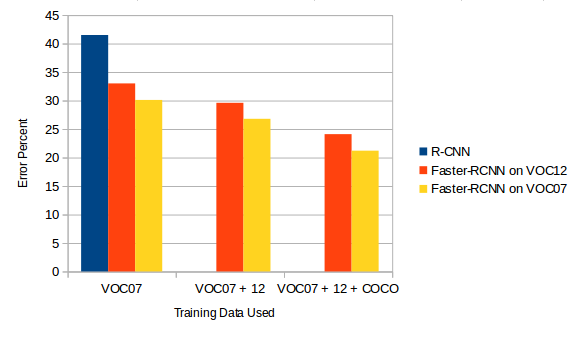
\includegraphics[width=14cm]{figs/data_vs_error.png}
\centering
\caption{Improvement of error as data increases, compared to error improvements due to algorithm improvements.
As we can see by comparing the drop from RCNN to Faster-RCNN on VOC07 only, and the drop from adding training data to Faster-RCNN, increasing data contributes significantly to error reduction.}
\end{figure}

Therefore, for real-world application development, data can be cheaper and more effective than scientists.
While many existing tools support image classification -- it is even built into Amazon Mechanical Turk (MTurk) -- and some tools support bounding box labeling in images, few tools exist for frame-by-frame labeling in videos.
VATIC~\cite{Vatic} stands out as being one of the best, as not only does it make high quality annotations one of its main goals, but also cost and scalability.

My work borrows and improves upon many concepts and results from VATIC's user studies, but I focus on an additional goal that is extremely important in creating datasets for real applications. That goal is researcher happiness.
Although VATIC extensively tested its ``User Interfaces'', I argue in chapter~\ref{chap:experimenter} that both the annotators and the experimenters are users, and the interfaces should be smooth for both when creating a tool.

Then, in chapter~\ref{chap:annotator}, I discuss my take on VATIC's User Interface principles for the annotator, and improvements upon them.

I also release all related code for BeaverDam, my video labeling platform, on Github.\footnote{http://github.com/antingshen/beaverdam} At time of writing, the library has been used by Berkeley Deep Drive, DeepScale, and BMW.

\section*{Related Work}
\label{sec:related}

There are a large number of static image annotators available.
For most computer vision applications that only require images instead of videos, these simpler alternatives should be used.
For bounding box annotations, crowdsourcing sites such as Mechanical Turk or Crowdflower may have templates providing such functionality.
For more complicated labels, tools such as LabelMe~\cite{LabelMe} provide many features for tasks such as image segmentation.
However, none of these tools provide the ability to easily label every frame of a video.

There exists some public datasets of labeled videos.
The YouTube-8M dataset~\cite{YouTube-8M} has millions of annotated videos, but they are annotated using the Inception V3 model trained on ImageNet.
The KITTI dataset~\cite{KITTI}, as well as a dataset being built at Berkeley Deep Drive, have labeled videos.
But these videos are not labeled every frame, instead an image is sampled every few seconds.
Those images are then labeled using static image annotators.
While these types of sampled image datasets are still useful, they don't allow research on supervised learning using nearby frames of a video, such as using an LSTM that uses each frame as input.

BeaverDam is designed to create frame-by-frame labeled video datasets.
Such existing datasets include VIRAT, a dataset created using VATIC~\cite{Vatic}.
However, labeling videos with existing tools is difficult and expensive, so these datasets are rarer and smaller.
Even setting up the first job is often a week-long project, consuming valuable researcher time.
Modifying them for each dataset's custom specifications is also difficult.
We created BeaverDam to address these problems.

